%--------------------------------------------------
% Artigo no template rbie2026 da Revista Brasileira de Informática na Educação.
% Preâmbulo baseado em template_oficial/main-pt.tex (não alterar a classe,
% o .bst nem as opções de \DocumentMetadata).
%
% Versão anônima (submissão):   make  (ou latexmk -lualatex main.tex)
% Versão identificada (final):  make identificado
%--------------------------------------------------

\DocumentMetadata{
  lang          = pt-BR,
  pdfversion    = 2.0,
  pdfstandard   = ua-2,
  tagging       = off
}

\documentclass[portuguese]{rbie2026}%

\usepackage[bottom]{footmisc}
\usepackage{tabularray}
\UseTblrLibrary{booktabs}
\usepackage{siunitx}
\usepackage{codehigh}
\usepackage{url}
\usepackage{xurl} % permite quebrar URLs longas em qualquer ponto (evita linhas estouradas nas referências)
\hyphenation{non-or-thog-o-nal}

\clubpenalty  = 100000000
\widowpenalty = 100000000

\graphicspath{{images/}}

% Versão identificada: definida por -usepretex='\def\versaoidentificada{}'
\newif\ifidentificado
\ifdefined\versaoidentificada \identificadotrue \fi

%----- HEADER INFORMATION. DO NOT EDIT -----------
%----- RESERVED FOR EDITORS ONLY
\jid{RBIE}
\jtitle{Revista Brasileira de Informática na Educação, 20XX, VV:1}
\issn{1414-5685 (print), 2317-6121 (online)}
\doi{10.5753/rbie.yyyy.id}
\copyrightstatement{This work is licensed under a Creative Commons Attribution 4.0 International License}
\jyear{20XX}

\category{Artigo de Pesquisa / Research Paper / Artículo de investigación}
%--------------------------------------------------


%----- ACESSIBILIDADE: metadados do PDF (texto simples) -----
\ifidentificado
\hypersetup{pdftitle={Fatores intracontextuais do desempenho no IDEB: segmentação socioeconômica e análise intragrupo nos municípios do Maranhão},
            pdfauthor={Darlon José Coqueiro; Orlando Donato Rocha Filho; Danúbia Soares Pires}}
\else
\hypersetup{pdftitle={Fatores intracontextuais do desempenho no IDEB: segmentação socioeconômica e análise intragrupo nos municípios do Maranhão},
            pdfauthor={Omitido para revisão}}
\fi


%----- PAPER TITLE -------------------------------
\title[Fatores intracontextuais do desempenho no IDEB]{Fatores intracontextuais do desempenho no IDEB: segmentação socioeconômica e análise intragrupo nos municípios do Maranhão}

\engtitle{\textcolor{engtitle}{Intracontextual factors of IDEB performance: socioeconomic segmentation and within-group analysis in the municipalities of Maranhão}}

\thirdlangtitle{\textcolor{thirdlangtitle}{Factores intracontextuales del desempeño en el IDEB: segmentación socioeconómica y análisis intragrupo en los municipios de Maranhão}}

% Título alternativo sugerido para a RBIE (não aprovado; o professor preferiu manter o original).
% pdftitle correspondente: Comparar o comparável: agrupamento K-Means e fatores escolares associados ao IDEB nos municípios do Maranhão
% \title[Agrupamento \textit{K-Means} e fatores escolares do IDEB]{Comparar o comparável: agrupamento \textit{K-Means} e fatores escolares associados ao IDEB nos municípios do Maranhão}

% \engtitle{\textcolor{engtitle}{Comparing like with like: K-Means clustering and school factors associated with IDEB in the municipalities of Maranhão, Brazil}}

% \thirdlangtitle{\textcolor{thirdlangtitle}{Comparar lo comparable: agrupamiento K-Means y factores escolares asociados al IDEB en los municipios de Maranhão, Brasil}}
%--------------------------------------------------


%----- AUTHOR INFORMATION ------------------------
\ifidentificado
\author[Coqueiro et al. 20XX]{
    \affil{\textbf{Darlon José Coqueiro} \thinspace \orcidlink{0009-0003-1296-9548} \thinspace \textcolor{blue}{\faEnvelopeO} \enspace [{Instituto Federal de Educação, Ciência e Tecnologia do Maranhão} \thinspace | \thinspace \href{mailto:darlon.coqueiro@ifma.edu.br}{{\textit{darlon.coqueiro@ifma.edu.br}}}]}
    \affil{\textbf{Orlando Donato Rocha Filho} \thinspace \orcidlink{0000-0001-5952-7139} \enspace [{Instituto Federal de Educação, Ciência e Tecnologia do Maranhão} \thinspace | \thinspace \href{mailto:orlando.rocha@ifma.edu.br}{{\textit{orlando.rocha@ifma.edu.br}}}]}
    \affil{\textbf{Danúbia Soares Pires} \thinspace \orcidlink{0000-0002-1307-7985} \enspace [{Instituto Federal de Educação, Ciência e Tecnologia do Maranhão} \thinspace | \thinspace \href{mailto:danubiapires@ifma.edu.br}{{\textit{danubiapires@ifma.edu.br}}}]}
}
\else
\author[Omitido para revisão]{\affil{Omitido para revisão}}
\fi

% Endereço de correspondência: só na versão identificada. Definido fora do
% frontmatter porque condicionais dentro dele quebram a compilação.
\ifidentificado
\newcommand{\blocomail}{\begin{mail}Instituto Federal de Educação, Ciência e Tecnologia do Maranhão (IFMA), São Luís, MA, Brasil.\end{mail}}
\else
\newcommand{\blocomail}{}
\fi
%--------------------------------------------------


\begin{document}

\begin{frontmatter}
    \maketitle

    \blocomail

    \begin{abstract-pt}
        \textit{Introdução.} O desempenho educacional dos municípios maranhenses está entre os mais baixos do país, e a desigualdade socioeconômica entre eles dificulta comparar redes de ensino diretamente. Comparações sem controle de contexto tendem a atribuir a fatores escolares diferenças que vêm da renda. \textit{Métodos.} O estudo, quantitativo e baseado em dados públicos, combina mineração de dados educacionais e estatística não paramétrica em dois estágios. No primeiro, o algoritmo \textit{K-Means} agrupa os 216 municípios do Maranhão com Índice de Desenvolvimento da Educação Básica (IDEB) 2025 divulgado, nos anos iniciais da rede municipal, pela renda \textit{per capita} e pela proporção de moradores em pobreza extrema do Censo Demográfico 2022. O número de grupos é escolhido pelo \textit{Silhouette Score} e confirmado por estabilidade \textit{bootstrap}. No segundo estágio, dentro de cada grupo, o teste de Mann-Whitney, com delta de Cliff e correção de Benjamini-Hochberg, compara os quartis superior e inferior de desempenho em doze variáveis do Censo Escolar 2025. \textit{Resultados.} A partição em três grupos foi a mais bem separada e a mais estável. Nos grupos de renda baixa e intermediária, os municípios de IDEB alto têm de 10 a 12 pontos percentuais a mais de docentes com ensino superior e com licenciatura, com efeito médio. No grupo intermediário, destaca-se também a presença de quadra esportiva. \textit{Discussão.} A formação docente é o fator escolar mais consistente entre os grupos, mas o poder preditivo conjunto das variáveis é baixo e o desenho é associativo. A segmentação prévia por agrupamento é um procedimento replicável para comparar redes de ensino em contextos semelhantes.
    \end{abstract-pt}

    \begin{pchaves}
        Mineração de Dados Educacionais; Agrupamento; K-Means; IDEB; Formação Docente; Eficácia Escolar.
    \end{pchaves}

    \begin{abstract-en}
        \textit{Introduction.} The educational performance of municipalities in Maranhão is among the lowest in Brazil, and socioeconomic inequality among them makes direct comparisons between school systems difficult. Comparisons that do not control for context tend to attribute to school factors differences that stem from income. \textit{Methods.} This quantitative study, based on public data, combines educational data mining and nonparametric statistics in two stages. In the first, the K-Means algorithm clusters the 216 municipalities of Maranhão with a released 2025 Basic Education Development Index (IDEB), for the early years of municipal elementary schools, by per capita income and the share of residents in extreme poverty from the 2022 Demographic Census. The number of clusters is chosen by the Silhouette Score and confirmed by bootstrap stability. In the second stage, within each cluster, the Mann-Whitney test, with Cliff's delta and Benjamini-Hochberg correction, compares the upper and lower performance quartiles on twelve variables from the 2025 School Census. \textit{Results.} The three-cluster partition was the best separated and the most stable. In the low- and middle-income clusters, high-IDEB municipalities have 10 to 12 percentage points more teachers with higher education and with a teaching degree, with a medium effect size. In the middle-income cluster, sports courts also stand out. \textit{Discussion.} Teacher education is the most consistent school factor across clusters, but the joint predictive power of the variables is low and the design is associative. Prior segmentation by clustering is a replicable procedure for comparing school systems in similar contexts.
    \end{abstract-en}

    \begin{keywords}
        Educational Data Mining; Clustering; K-Means; IDEB; Teacher Education; School Effectiveness.
    \end{keywords}

    \begin{abstract-es}
        \textit{Introducción.} El desempeño educativo de los municipios de Maranhão está entre los más bajos de Brasil, y la desigualdad socioeconómica entre ellos dificulta comparar directamente las redes de enseñanza. Las comparaciones sin control del contexto tienden a atribuir a factores escolares diferencias que provienen de la renta. \textit{Métodos.} El estudio, cuantitativo y basado en datos públicos, combina minería de datos educativos y estadística no paramétrica en dos etapas. En la primera, el algoritmo K-Means agrupa los 216 municipios de Maranhão con Índice de Desarrollo de la Educación Básica (IDEB) 2025 divulgado, en los años iniciales de la red municipal, por la renta \textit{per cápita} y la proporción de residentes en pobreza extrema del Censo Demográfico 2022. El número de grupos se elige por el \textit{Silhouette Score} y se confirma por estabilidad \textit{bootstrap}. En la segunda etapa, dentro de cada grupo, la prueba de Mann-Whitney, con delta de Cliff y corrección de Benjamini-Hochberg, compara los cuartiles superior e inferior de desempeño en doce variables del Censo Escolar 2025. \textit{Resultados.} La partición en tres grupos fue la mejor separada y la más estable. En los grupos de renta baja e intermedia, los municipios de IDEB alto tienen de 10 a 12 puntos porcentuales más de docentes con educación superior y con licenciatura, con efecto medio. En el grupo intermedio, destacan también las canchas deportivas. \textit{Discusión.} La formación docente es el factor escolar más consistente entre los grupos, pero el poder predictivo conjunto de las variables es bajo y el diseño es asociativo. La segmentación previa por agrupamiento es un procedimiento replicable para comparar redes de enseñanza en contextos semejantes.
    \end{abstract-es}

    \begin{pclaves}
        Minería de Datos Educativos; Agrupamiento; K-Means; IDEB; Formación Docente; Eficacia Escolar.
    \end{pclaves}

    \begin{dates}
        {\sffamily\textbf{Received:}} DD Month YYYY \enspace\textbullet\enspace
        {\sffamily\textbf{Accepted:}} DD Month YYYY \enspace\textbullet\enspace
        {\sffamily\textbf{Published:}} DD Month YYYY
    \end{dates}

\end{frontmatter}

\section{Introdução}
\label{sec:intro}

A qualidade da educação básica é um dos principais determinantes do desenvolvimento humano e econômico de longo prazo \citep{hanushek2012}. No Brasil, o Índice de Desenvolvimento da Educação Básica (IDEB) monitora o ensino público combinando fluxo escolar e proficiência em língua portuguesa e matemática numa medida comparável entre municípios, estados e redes de ensino \citep{fernandes2007}. Apesar dos avanços das últimas duas décadas, as disparidades regionais persistem: estados do Norte e do Nordeste ficam sistematicamente abaixo da média nacional, reflexo de desigualdades estruturais de renda, infraestrutura e serviços públicos \citep{inep2025}.

O Maranhão está entre os casos mais críticos. Com a menor renda domiciliar \textit{per capita} do país no Censo Demográfico 2022 e indicadores educacionais historicamente abaixo da média nacional, o estado concentra municípios em alta vulnerabilidade socioeconômica \citep{ibge2022, inep2025}. Ainda assim, o desempenho varia entre municípios de condições semelhantes, o que coloca uma pergunta direta: o que diferencia, dentro de um mesmo patamar de vulnerabilidade, os municípios de maior IDEB daqueles de menor IDEB?

A literatura internacional examinou amplamente a relação entre condições socioeconômicas, infraestrutura escolar, qualificação docente e o desempenho dos estudantes \citep{rivkin2005, coleman1966}. No Brasil, a pesquisa em eficácia escolar mostrou que o nível socioeconômico dos alunos é o fator mais associado ao desempenho, mas que as escolas também fazem diferença \citep{brooke2008}. Estudos com dados do IDEB e do Censo Escolar associaram o desempenho à infraestrutura e à complexidade das escolas \citep{alves2013, vasconcelos2021}. Já a formação específica em licenciatura dos professores da educação básica permanece como meta nacional ainda não cumprida \citep{brasil2014, gatti2019}. Análises voltadas especificamente para o Maranhão que isolem fatores intracontextuais (aqueles que se mantêm associados ao desempenho mesmo entre municípios de contexto socioeconômico semelhante) são escassas.

Métodos de aprendizado de máquina têm sido aplicados a dados educacionais com resultados promissores, especialmente pela capacidade de lidar com bases administrativas grandes e heterogêneas \citep{ersozlu2024, kalita2025, romero2020}. Algoritmos de agrupamento identificam estruturas nos dados sem categorias predefinidas, o que os torna úteis para segmentar contextos antes de comparações \citep{faceli2021, kalita2025}. Quando a segmentação é seguida de testes não paramétricos aplicados dentro de cada grupo, torna-se possível comparar municípios de desempenho distinto sem confundir fatores escolares com diferenças de contexto.

O objetivo geral deste artigo é identificar, entre municípios maranhenses de contexto socioeconômico semelhante, os fatores escolares associados ao desempenho superior no IDEB 2025 dos anos iniciais do ensino fundamental da rede municipal. Duas questões de pesquisa (QP) orientam o estudo:

\begin{description}
    \item[QP1.] Em quantos grupos socioeconômicos os municípios maranhenses se organizam, considerando a renda \textit{per capita} e a pobreza extrema, e quão estável é essa partição?
    \item[QP2.] Dentro de cada grupo, quais fatores de infraestrutura, qualificação docente e fluxo escolar diferenciam os municípios de alto e de baixo IDEB?
\end{description}

Para respondê-las, a análise abrange os 216 municípios maranhenses com IDEB 2025 divulgado, de um total de 217, em dois estágios. No primeiro, os municípios são agrupados por contexto socioeconômico via \textit{K-Means}, usando a renda \textit{per capita} e a proporção de moradores em pobreza extrema, ambas do Censo Demográfico 2022. No segundo, dentro de cada grupo, o teste de Mann-Whitney, acompanhado de tamanho de efeito e de correção para comparações múltiplas, identifica quais características escolares e socioeconômicas diferem entre municípios de alto e baixo desempenho. As variáveis analisadas vêm do Censo Escolar 2025: infraestrutura (internet, biblioteca, laboratório de informática, saneamento), qualificação docente e indicadores de fluxo escolar.

O trabalho faz três contribuições principais. Primeiro, identifica os fatores escolares associados ao desempenho superior no IDEB dentro de cada perfil socioeconômico, tanto no grupo de municípios mais vulneráveis quanto no de renda intermediária, com destaque para a formação docente. Segundo, oferece evidência sobre o Maranhão, estado pouco estudado nessa literatura e no qual a comparação direta com médias nacionais é pouco informativa. Terceiro, aplica uma abordagem em dois estágios (segmentação socioeconômica seguida de análise intragrupo), construída com dados públicos e \textit{scripts} abertos, que pode ser replicada em outras unidades federativas. Os resultados oferecem subsídios a gestores e formuladores de políticas que precisam decidir onde concentrar recursos.

O restante do artigo está organizado da seguinte forma. A Seção~\ref{sec:relacionados} apresenta o referencial teórico sobre os fatores associados ao desempenho no IDEB e sobre a mineração de dados educacionais, e posiciona o estudo em relação aos trabalhos relacionados. A Seção~\ref{sec:metodos} descreve as fontes de dados, as variáveis e os dois estágios da análise. A Seção~\ref{sec:resultados} apresenta a segmentação dos municípios e os fatores discriminantes, organizados pelas questões de pesquisa e discutidos à luz da literatura. A Seção~\ref{sec:limitations} discute as limitações, e a Seção~\ref{sec:conclusion} sintetiza os achados e aponta trabalhos futuros.

\section{Referencial Teórico e Trabalhos Relacionados}
\label{sec:relacionados}

Compreender os fatores associados ao desempenho escolar exige articular dois campos de conhecimento: os estudos educacionais sobre os fatores associados ao desempenho e os métodos computacionais capazes de extrair padrões de grandes bases administrativas. Esta seção reúne essas bases, que sustentam as escolhas metodológicas e a interpretação dos resultados. Inicialmente, apresentam-se os estudos sobre o IDEB e os fatores associados ao desempenho escolar, com atenção à formação docente e à escassez de pesquisas voltadas ao Maranhão. Em seguida, discutem-se a mineração de dados educacionais e o agrupamento não supervisionado como estratégia de segmentação contextual. Por fim, delimita-se a contribuição deste estudo em relação a essa literatura.

\subsection{O IDEB e os fatores associados ao desempenho escolar no Brasil}

O IDEB foi concebido por \citet{fernandes2007} como uma medida composta que combina taxa de aprovação (fluxo) e proficiência em Língua Portuguesa e Matemática aferida pelo Sistema de Avaliação da Educação Básica (Saeb), resultando em um indicador comparável ao longo do tempo e entre redes de ensino. \citet{soares2013} examinaram os pressupostos estatísticos do índice, alertando para o risco de interpretações simplistas que ignoram a correlação entre fluxo e proficiência.

A relação entre a qualidade do professor e o desempenho escolar é um dos achados mais robustos da literatura internacional. \citet{rivkin2005}, em análise com dados do Texas, demonstraram que a qualidade do professor é o fator intraescolar com maior impacto sobre o aprendizado dos estudantes, superando o tamanho de turma. Os mesmos autores observaram, porém, que características observáveis dos docentes, como a titulação, explicam pouco dessa variação. A evidência sobre a titulação formal é, portanto, menos consistente do que a evidência sobre a qualidade do professor, o que torna relevante verificar se ela se associa ao desempenho em redes nas quais parte expressiva dos docentes ainda não tem formação superior. O efeito-escola, por sua vez, é discutido desde o clássico relatório de \citet{coleman1966}, que identificou nos Estados Unidos que o contexto socioeconômico familiar explica a maior parte da variância no desempenho, enquanto fatores escolares têm efeito residual (embora real e acionável por políticas públicas). No Brasil, a pesquisa em eficácia escolar, sistematizada por \citet{brooke2008}, retomou essa pergunta e mostrou que, controlado o nível socioeconômico dos alunos, as escolas ainda diferem entre si no quanto seus estudantes aprendem.

No campo da formação docente, a Meta 15 do Plano Nacional de Educação estabelece que todos os professores da educação básica tenham formação específica de nível superior, obtida em curso de licenciatura na área de conhecimento em que atuam \citep{brasil2014}. \citet{gatti2019} analisam o cenário da formação de professores no país, marcado pela expansão das licenciaturas, sobretudo a distância, e pela persistência de docentes em exercício sem a formação exigida. É nesse quadro que a proporção de docentes com licenciatura, variável analisada neste estudo, ganha interesse como indicador acompanhado pela política educacional.

\citet{albernaz2002} identificaram que qualidade e equidade no ensino fundamental variam sistematicamente com o nível socioeconômico das escolas, evidenciando que comparações entre municípios de contextos distintos tendem a confundir efeito-escola com efeito-contexto. \citet{alves2013} mostraram que o IDEB das escolas varia com o nível socioeconômico dos alunos, a infraestrutura e a complexidade da escola, e que a associação com a infraestrutura é mais forte nos anos iniciais do ensino fundamental, a etapa analisada neste estudo. \citet{vasconcelos2021} construíram um índice de infraestrutura escolar para os municípios brasileiros, com dados do Censo Escolar de 2007 e 2017, e, por regressão quantílica, encontraram que a infraestrutura tem maior importância para o IDEB do que o volume de investimento público em educação. Em revisão dos estudos publicados entre 1990 e 2010 sobre recursos escolares em países em desenvolvimento, \citet{glewwe2013} verificaram que a maioria das características de escolas e professores não tem efeito estatisticamente significativo sobre o aprendizado quando se consideram apenas os estudos metodologicamente mais rigorosos. Entre as exceções estão o conhecimento do professor sobre a disciplina que leciona, a ausência docente (com efeito negativo), as bibliotecas e a qualidade das instalações físicas; a escolaridade do professor, associada positivamente ao aprendizado no conjunto amplo de estudos, não mostrou efeito consistente no subconjunto de maior rigor. \citet{hanushek2012} demonstraram, em perspectiva comparada entre países, que habilidades cognitivas têm efeito causal sobre crescimento econômico de longo prazo, reforçando a relevância de investigar os fatores associados ao desempenho escolar em estados de baixa renda, como o Maranhão.

Na literatura consultada para este estudo, análises centradas especificamente no Maranhão são escassas. O estado figurou sistematicamente entre os piores índices nacionais no IDEB das séries iniciais \citep{inep2025}, com média municipal de 5,4 nos anos iniciais na edição mais recente. A concentração de municípios em condições de alta vulnerabilidade socioeconômica torna necessária uma abordagem que controle o contexto antes de comparar desempenhos, cuidado que nem sempre está presente em análises aplicadas ao conjunto dos municípios do país.

\subsection{Mineração de dados educacionais}

A mineração de dados educacionais (\textit{Educational Data Mining}, EDM) consolidou-se como área de pesquisa a partir da segunda metade da década de 2000, quando \citet{baker2010} mapearam o estado da arte e identificaram cinco grandes paradigmas: predição, agrupamento, mineração de regras de associação, descoberta com modelos e visualização. Em revisão atualizada, \citet{romero2020} estenderam esse panorama e evidenciaram a predominância de técnicas supervisionadas para tarefas de classificação, especialmente para predizer aprovação, evasão e desempenho em avaliações padronizadas.

No Brasil, a aplicação de algoritmos de aprendizado supervisionado a dados administrativos educacionais ganhou tração com a ampla disponibilização de microdados do Instituto Nacional de Estudos e Pesquisas Educacionais Anísio Teixeira (INEP). Estudos baseados no Censo Escolar e no IDEB aplicaram técnicas de mineração de dados para identificar fatores associados a desempenho e evasão \citep{colpani2018}. A capacidade dessas técnicas de lidar com bases de alta dimensionalidade e distribuições assimétricas as torna adequadas a dados como os do Censo Escolar, que apresentam essas características.

Na literatura consultada, observam-se três limitações recorrentes, que motivam o desenho deste estudo: a menor presença de estudos voltados aos estados do Norte e do Nordeste; o uso de modelos globais, que tratam municípios de contextos socioeconômicos muito distintos como comparáveis; e a sub-representação de estados como o Maranhão, onde as condições de vulnerabilidade tornam pouco informativa a comparação direta com médias nacionais.

\subsection{Aprendizado não supervisionado para segmentação contextual}

O agrupamento (\textit{clustering}) via \textit{K-Means}, proposto por \citet{macqueen1967}, é uma das técnicas de aprendizado não supervisionado mais amplamente utilizadas para segmentação de entidades em grupos homogêneos internamente e heterogêneos entre si \citep{faceli2021}. O algoritmo minimiza a inércia intragrupo por meio de iterações de atribuição e recentramento, requerendo apenas a especificação prévia do número de grupos~$k$.

A seleção de $k$ é um desafio clássico. O Método do Cotovelo (\textit{Elbow Method}) avalia a variação da inércia, mas pode ser ambíguo em dados reais. O \textit{Silhouette Score}, introduzido por \citet{rousseeuw1987}, oferece uma métrica mais interpretável. Para cada ponto, ele compara a coesão com o próprio grupo e a separação em relação ao \textit{cluster} mais próximo. O resultado é um escore entre $-1$ e 1: quanto mais alto, mais bem definido o agrupamento. A estabilidade da partição sob reamostragem, proposta por \citet{benhur2002}, é um critério complementar: uma partição que reflete estrutura real dos dados tende a se repetir quando o algoritmo é executado sobre subamostras.

Em contextos educacionais, técnicas de agrupamento, como o \textit{K-Means}, têm sido empregadas para identificar grupos de escolas com características socioeconômicas semelhantes. No contexto brasileiro, \citet{alves2014} utilizaram análise de conglomerados pelo método \textit{K-Means} para agrupar as escolas de educação básica em sete níveis segundo seu índice socioeconômico, estabelecendo grupos com diferentes perfis de contexto social. Essa abordagem demonstra o potencial de técnicas de clusterização para caracterizar e segmentar unidades educacionais a partir de indicadores socioeconômicos, possibilitando análises posteriores das diferenças entre os grupos em outros indicadores educacionais.

A visualização dos \textit{clusters} via Análise de Componentes Principais (\textit{Principal Component Analysis}, PCA) \citep{abdi2010} permite inspecionar graficamente a qualidade da separação em espaço bidimensional, mesmo quando as variáveis originais têm escalas incomparáveis.

Combinar a segmentação por \textit{K-Means} com testes aplicados dentro de cada grupo torna as comparações mais equilibradas. Ao comparar municípios dentro do mesmo \textit{cluster} socioeconômico, reduz-se, sem eliminar, o risco de atribuir a fatores escolares diferenças que são, na verdade, determinadas pela renda ou pela concentração de pobreza.

\subsection{Posicionamento deste estudo}

Os estudos sobre fatores associados ao IDEB tratam o nível socioeconômico como mais uma variável explicativa, ao lado dos fatores escolares \citep{alves2013}. Quando o agrupamento aparece, ele costuma ser o próprio produto da análise, como nos níveis socioeconômicos de \citet{alves2014}. O presente trabalho usa o agrupamento como meio, e distingue-se da literatura existente por três características:

\begin{enumerate}[label=\alph*)]
    \item adota uma abordagem em dois estágios que separa explicitamente a segmentação socioeconômica da análise de fatores intracontextuais, sem exigir que se suponha uma forma funcional para a relação entre contexto e desempenho;
    \item aplica essa lógica exclusivamente aos municípios maranhenses (216 dos 217, os que têm IDEB 2025 divulgado), contexto sub-representado na literatura de EDM;
    \item complementa os testes de Mann-Whitney \citep{mannwhitney1947} com tamanho de efeito, controle da taxa de falsas descobertas e verificação do poder preditivo das variáveis, o que permite distinguir associações pontuais de fatores com capacidade explicativa.
\end{enumerate}

A análise intragrupo, restrita a municípios com contexto socioeconômico semelhante, responde a uma pergunta que modelos globais deixam em aberto: quais fatores diferem, de forma consistente e estatisticamente significativa, entre os municípios de maior e de menor IDEB dentro de um mesmo patamar socioeconômico? Essa pergunta interessa às políticas educacionais porque aponta candidatos a intervenção que se mantêm associados ao desempenho mesmo sob restrições socioeconômicas semelhantes.

\section{Metodologia}
\label{sec:metodos}

Trata-se de uma pesquisa de abordagem quantitativa e, quanto aos objetivos, descritiva, na acepção de \citet{gil2017}: busca descrever as características de uma população (os municípios maranhenses) e estabelecer relações entre variáveis, sem manipulá-las. Quanto aos procedimentos técnicos, classifica-se como pesquisa documental \citep{gil2017}, pois utiliza exclusivamente dados secundários de acesso público, produzidos pelo INEP e pelo Instituto Brasileiro de Geografia e Estatística (IBGE) com outras finalidades e aqui reanalisados. O \textit{pipeline} analítico segue as etapas do processo CRISP-DM (\textit{Cross-Industry Standard Process for Data Mining}) \citep{shearer2000}, adaptado ao contexto de análise de dados educacionais: compreensão do domínio, coleta e preparação dos dados, modelagem e avaliação dos resultados. Dentro desse processo, a análise é conduzida em dois estágios sequenciais, resumidos na Figura~\ref{fig:fluxo}: o primeiro responde à QP1 e o segundo, à QP2.

\begin{figure}[!ht]
    \centering
    \small
    \fbox{\parbox{0.92\linewidth}{\centering
        \textbf{Dados}: IDEB 2025 $+$ Censo Escolar 2025 $+$ Censo Demográfico 2022\\[2pt]
        $\downarrow$ integração por município (n = 216)\\[2pt]
        \textbf{Estágio 1 (QP1)}: \textit{K-Means} sobre renda e pobreza extrema;\\ escolha de $k$ por \textit{Silhouette}, estabilidade e ablação\\[2pt]
        $\downarrow$ \textit{clusters} socioeconômicos\\[2pt]
        \textbf{Estágio 2 (QP2)}: em cada \textit{cluster}, quartil superior $\times$ inferior de IDEB;\\ Mann-Whitney, $\delta$ de Cliff, valor $q$, Spearman e validação preditiva
    }}
    \caption{Desenho da análise em dois estágios. Fonte: elaboração própria.}
    \label{fig:fluxo}
\end{figure}

\subsection{Fontes de dados}

Este estudo integra três bases de dados públicas referentes aos municípios do Maranhão:

\begin{itemize}
    \item \textbf{IDEB EFAI 2025 (INEP).} O IDEB dos anos iniciais do ensino fundamental (EFAI), divulgado pelo \citet{inep2025}, é calculado conforme a metodologia proposta por \citet{fernandes2007}: combina a taxa de aprovação escolar (fluxo) com a proficiência média em Língua Portuguesa e Matemática aferida pelo Saeb. Para este estudo, utilizou-se a edição 2025 da rede municipal, que cobriu 216 dos 217 municípios do estado; Nova Iorque não teve o indicador divulgado nesta edição, porque o INEP não divulgou as notas do município no Saeb.

    \item \textbf{Censo Escolar 2025 (INEP).} Os microdados do Censo Escolar \citep{inep2026microdados} fornecem informações em nível de escola sobre infraestrutura física (internet, biblioteca ou sala de leitura, laboratório de informática, quadra esportiva, abastecimento de água e esgotamento sanitário) e sobre o corpo docente. Para as variáveis de formação docente nos anos iniciais, utilizou-se a Tabela 2.29 da Sinopse Estatística da Educação Básica 2025 \citep{inep2026sinopse}. Ela fornece o número de docentes EFAI por nível de formação com numerador e denominador consistentes, sem a dupla contagem presente nos microdados brutos.

    \item \textbf{Censo Demográfico 2022 (IBGE).} Do Censo Demográfico 2022 do IBGE foram extraídas duas medidas municipais de renda domiciliar \textit{per capita}. A primeira é o valor do rendimento nominal médio mensal domiciliar \textit{per capita} (Sistema IBGE de Recuperação Automática, Sidra, tabela 10295) \citep{ibge2022}; a segunda, a distribuição dos moradores por classes de rendimento domiciliar \textit{per capita} em salários mínimos (Sidra, tabela 10296) \citep{ibge2022classes}. Por ser um recenseamento, e não uma pesquisa amostral, o Censo Demográfico é a única fonte de renda com cobertura de todos os 217 municípios do estado.
\end{itemize}

\subsection{Variáveis de segmentação socioeconômica}

A segmentação dos municípios utiliza duas variáveis, ambas do Censo Demográfico 2022:

\begin{itemize}
    \item \textbf{Renda \textit{per capita}}: rendimento nominal médio mensal domiciliar \textit{per capita}, em reais. Mede o \emph{nível} de recursos econômicos disponíveis no município.
    \item \textbf{Pobreza extrema}: percentual de moradores em domicílios com rendimento \textit{per capita} de até 1/4 do salário mínimo ou sem rendimento. Mede a \emph{concentração} de famílias em privação severa. O corte de 1/4 do salário mínimo é o critério de miserabilidade adotado pela Lei Orgânica da Assistência Social para o Benefício de Prestação Continuada \citep{brasil1993}, o que o torna uma linha de referência institucional reconhecida no Brasil.
\end{itemize}

A escolha dessas duas variáveis apoia-se em três argumentos. O primeiro é teórico: o nível socioeconômico é o preditor mais consistente do desempenho escolar desde \citet{coleman1966}, e a meta-análise de \citet{sirin2005} mostra que essa associação é mais forte quando medida em unidades agregadas, como escolas e distritos, do que no nível individual. Controlar o contexto socioeconômico dos municípios antes de comparar seu desempenho é, portanto, condição para não atribuir a fatores escolares diferenças que decorrem da renda \citep{albernaz2002}. O segundo argumento é que as duas medidas captam aspectos complementares da renda: a média é sensível a rendas altas concentradas em poucos domicílios, enquanto a proporção de moradores em pobreza extrema descreve a base da distribuição. Dois municípios com renda média semelhante podem ter proporções bastante diferentes de famílias em privação severa. O terceiro argumento é de consistência temporal: ambas vêm do mesmo recenseamento, de 2022, o mais recente com desagregação municipal completa.

As duas variáveis são correlacionadas (coeficiente de Pearson de $-0{,}87$ entre os 216 municípios analisados), o que é esperado, dado que ambas derivam da distribuição de renda. A contribuição de cada uma para a partição é avaliada no Estágio 1 por meio de um teste de ablação, que refaz a clusterização sem cada variável e mede o quanto a partição se altera.

\subsection{Variáveis}

O conjunto completo de variáveis é organizado em quatro grupos, descritos na Tabela~\ref{tab:variaveis}.

\begin{table*}[!ht]
    \caption{Variáveis utilizadas na análise. As variáveis escolares referem-se à rede municipal e são agregadas por município. Fonte dos dados: Censo Demográfico 2022 (IBGE), Censo Escolar 2025 e Sinopse Estatística 2025 (INEP).}
    \label{tab:variaveis}
    \centering
    \begin{tblr}{%
        colspec = {X[1.1,l] X[0.45,l] X[1.6,l]},
        cells   = {font=\small},
        row{1}  = {font=\small\bfseries},
        width   = 0.92\linewidth
        }
        \toprule
        Variável & Fonte & Definição operacional \\
        \midrule
        \SetCell[c=3]{l}{\textit{Segmentação socioeconômica}} & & \\
        Renda \textit{per capita} & Censo 2022 & Rendimento domiciliar \textit{per capita} médio mensal municipal (R\$) \\
        Pobreza extrema & Censo 2022 & \% de moradores com rendimento domiciliar \textit{per capita} de até 1/4 do salário mínimo ou sem rendimento \\
        \midrule
        \SetCell[c=3]{l}{\textit{Infraestrutura escolar}} & & \\
        \% escolas com internet & Censo 2025 & Proporção de escolas municipais com acesso à internet \\
        \% escolas com biblioteca ou sala de leitura & Censo 2025 & Proporção com biblioteca, biblioteca-sala de leitura ou sala de leitura \\
        \% escolas com laboratório de informática & Censo 2025 & Proporção com laboratório de informática \\
        \% escolas com quadra esportiva & Censo 2025 & Proporção com quadra de esportes \\
        \% escolas com água adequada & Censo 2025 & Proporção com água potável ou rede pública \\
        \% escolas com esgoto adequado & Censo 2025 & Proporção com rede pública ou fossa séptica \\
        \midrule
        \SetCell[c=3]{l}{\textit{Qualificação docente}} & & \\
        \% docentes EFAI com ensino superior & Sinopse 2025 & Proporção de docentes dos anos iniciais com graduação \\
        \% docentes EFAI com licenciatura & Sinopse 2025 & Proporção de docentes dos anos iniciais com licenciatura \\
        \midrule
        \SetCell[c=3]{l}{\textit{Fluxo e distorção}} & & \\
        Média de alunos por turma (educação básica) & Censo 2025 & Total de matrículas da educação básica dividido pelo total de turmas da educação básica \\
        Média de alunos por turma (ensino fundamental) & Censo 2025 & Total de matrículas no ensino fundamental dividido pelo total de turmas do ensino fundamental \\
        \textit{Proxy} de distorção idade-série & Censo 2025 & \% de matrículas com 15 anos ou mais na educação básica municipal \\
        \% turmas com correção de fluxo (anos finais) & Censo 2025 & Proporção de turmas de correção de fluxo entre as turmas dos anos finais do ensino fundamental \\
        \bottomrule
    \end{tblr}
\end{table*}

\subsection{Coleta e pré-processamento dos dados}

A coleta e o tratamento dos dados foram automatizados em \textit{scripts} Python, organizados em três etapas (ingestão, transformação e análise), o que permite reproduzir integralmente a análise. Das três fontes, foram mantidas apenas as informações da rede municipal do Maranhão. No IDEB, os resultados não divulgados pelo INEP foram tratados como valores ausentes. No Censo Escolar, as informações de escola, docente, matrícula e turma foram combinadas escola a escola. Para os docentes dos anos iniciais, usou-se exclusivamente a Sinopse Estatística, de modo que o numerador (docentes com ensino superior ou licenciatura) e o denominador (total de docentes dos anos iniciais) viessem da mesma fonte. Os dados de renda e de pobreza extrema foram obtidos das tabelas do Sidra e armazenados localmente, para que a análise não dependa de alterações posteriores nas bases on-line.

As variáveis de infraestrutura foram agregadas ao nível municipal como proporção de escolas com cada atributo presente; as de docentes, como percentual sobre o total de docentes dos anos iniciais do município; e as de fluxo, como médias ou proporções sobre o total de matrículas e turmas municipais. A unidade de análise é, portanto, o município: as associações encontradas referem-se às redes municipais e não podem ser transpostas para escolas, professores ou alunos individualmente \citep{robinson1950}.

A Tabela 2.29 da Sinopse conta os docentes dos anos iniciais de todas as redes do município (municipal, estadual, federal e privada), enquanto o IDEB analisado é o da rede municipal. Nos \textit{clusters} em que se faz a comparação intragrupo, a rede municipal reúne, em média, 93\% (intermediário) e 95\% (vulnerável) dos docentes dos anos iniciais. Para verificar se esse descompasso afeta os resultados, a formação docente também foi calculada apenas na rede municipal, a partir dos microdados; como os microdados não separam a formação docente por etapa, essa medida abrange toda a educação básica municipal. As três bases foram então integradas por município, resultando em 217 municípios com renda, pobreza extrema e Censo Escolar completos, dos quais 216 têm o IDEB divulgado.

Não há valores ausentes nas variáveis de segmentação nem nas variáveis explicativas; municípios sem turmas de correção de fluxo aparecem com proporção zero nessa variável. A variável-alvo (IDEB) tem um valor ausente (Nova Iorque). Como o município não pode ser classificado por desempenho, ele é excluído dos dois estágios, e a análise segue com 216 municípios.

\subsection{Estágio 1: segmentação socioeconômica por \textit{K-Means}}

O \textit{K-Means} \citep{macqueen1967} agrupa os 216 municípios com base na renda \textit{per capita} e na pobreza extrema. Antes da clusterização, as duas variáveis são padronizadas pela mediana e pelo intervalo interquartil. Essa padronização reduz a influência de municípios atípicos, como São Luís e Imperatriz, cuja renda \textit{per capita} muito acima e pobreza extrema muito abaixo dos demais poderiam distorcer a formação dos grupos.

O algoritmo é executado para um número de grupos $k$ entre 2 e 10, com dez inicializações por valor de $k$ e semente fixa, o que torna o resultado reprodutível. O número de \textit{clusters} é escolhido pelo \textit{Silhouette Score} médio \citep{rousseeuw1987}, que mede a separação relativa dos grupos. A escolha é confirmada pela estabilidade da partição, avaliada por \textit{bootstrap} de 25 iterações com 80\% dos dados, na configuração de referência de \citet{benhur2002}, com o \textit{Adjusted Rand Index} (ARI) como métrica de concordância. A curva de inércia (Método do Cotovelo) é apresentada como apoio visual. A contribuição de cada variável é medida por ablação: a clusterização é refeita sem a variável, e o ARI entre a nova partição e a original indica o quanto a partição depende dela.

A visualização dos \textit{clusters} é feita via PCA \citep{abdi2010} com duas componentes, permitindo inspeção gráfica da separação em espaço reduzido.

\subsection{Estágio 2: análise intragrupo}

Dentro de cada \textit{cluster} com amostra suficiente, os municípios são divididos em dois grupos por desempenho: \textit{alto IDEB}, formado pelo quartil superior ($\geq Q_{75}$), e \textit{baixo IDEB}, formado pelo quartil inferior ($\leq Q_{25}$). Os municípios do intervalo central são excluídos da análise comparativa, o que aumenta o contraste entre os grupos e reduz o ruído. Exige-se um mínimo de dez municípios em cada extremo.

Para cada variável, o teste de Mann-Whitney \citep{mannwhitney1947} bicaudal verifica se as distribuições diferem entre os grupos de alto e de baixo IDEB. A magnitude da diferença é medida pelo $\delta$ de Cliff \citep{cliff1993}, que varia de $-1$ a $1$. Ele indica a probabilidade de um município do grupo alto apresentar valor maior que um do grupo baixo, descontada a probabilidade inversa. Seguindo \citet{vargha2000}, valores absolutos a partir de 0,12, 0,28 e 0,42 são lidos como efeitos pequeno, médio e grande. Como são testadas catorze variáveis em cada \textit{cluster}, os valores de $p$ são acompanhados do valor $q$ de \citet{benjamini1995}, que controla a taxa de falsas descobertas entre os testes. São reportadas as variáveis com $p < 0{,}10$, e a interpretação considera conjuntamente o valor $q$, a magnitude do efeito e a consistência do resultado entre os \textit{clusters}. Por essa razão, e pelo tamanho das amostras, o Estágio 2 tem caráter exploratório.

Duas verificações complementam a comparação, além da medida alternativa de formação docente descrita na seção anterior. A primeira, de robustez, calcula a correlação de Spearman entre cada variável e o IDEB usando todos os municípios do \textit{cluster}, sem descartar o intervalo central, o que testa se as associações dependem do corte por quartis. A segunda avalia o poder preditivo conjunto das variáveis, por validação cruzada em cinco partes repetida vinte vezes. Um classificador \textit{Random Forest} \citep{breiman2001}, com 500 árvores e ponderação das classes, tenta separar os grupos de alto e de baixo IDEB; seu desempenho é medido pela área sob a curva característica de operação do receptor (\textit{Receiver Operating Characteristic}, ROC), abreviada como AUC, em que 0,5 corresponde ao acaso. Uma regressão \textit{ridge} \citep{hoerl1970} tenta prever o IDEB contínuo, no estado e em cada \textit{cluster}; seu desempenho é medido pelo coeficiente de determinação ($R^2$) fora da amostra. As análises usam as bibliotecas pandas, SciPy e scikit-learn.

\subsection{Aspectos éticos}

O estudo usa apenas dados secundários de acesso público, agregados por município e sem possibilidade de identificação de pessoas. Por isso, dispensa apreciação pelo sistema de Comitês de Ética em Pesquisa, nos termos do art.~1º, parágrafo único, da Resolução CNS n.º 510/2016 \citep{cns2016resolucao510}.

\section{Análise e Discussão dos Resultados}
\label{sec:resultados}

Esta seção apresenta os resultados obtidos com a aplicação dos dois estágios descritos na metodologia e os discute à luz da literatura. Inicialmente, caracterizam-se o contexto socioeconômico e educacional do Maranhão e a distribuição do IDEB entre os municípios, o que evidencia a variabilidade de desempenho que motiva a investigação. Em seguida, responde-se à QP1, com a segmentação socioeconômica obtida com o \textit{K-Means}, e à QP2, com os fatores que diferenciam os municípios de alto e de baixo desempenho dentro de cada grupo com amostra suficiente. Por fim, esses achados são confrontados com a literatura e traduzidos em implicações para as políticas educacionais.

\subsection{Contexto socioeconômico e educacional do Maranhão}

O Maranhão é o segundo maior estado do Nordeste em extensão territorial e um dos mais populosos, com 217 municípios distribuídos em cinco mesorregiões. No Censo Demográfico 2022, o estado tem a menor renda domiciliar \textit{per capita} entre as 27 unidades da federação (R\$~899,87, contra R\$~1.638,06 no Brasil) \citep{ibge2022}. Tem também a segunda maior proporção de moradores em pobreza extrema, isto é, com rendimento \textit{per capita} de até 1/4 do salário mínimo ou sem rendimento (26,6\%, contra 13,3\% no Brasil) \citep{ibge2022classes}. Entre os municípios, a desigualdade também é expressiva: a renda \textit{per capita} mediana é de R\$~667, e a proporção de moradores em pobreza extrema varia de 11,2\% a 60,3\%. Esse contexto reflete-se nos resultados educacionais.

A Figura~\ref{fig:dist_ideb} apresenta a distribuição do IDEB dos 216 municípios com indicador divulgado. A distribuição é aproximadamente unimodal, ligeiramente assimétrica à direita, com média de 5,39 (desvio-padrão de 0,59), mediana de 5,30, mínimo de 4,10 e máximo de 8,10. A cauda superior é rarefeita: apenas 11 municípios atingem 6,50, e o máximo de 8,10 está um ponto acima do segundo maior valor (7,10).

\begin{figure}[!ht]
    \centering
    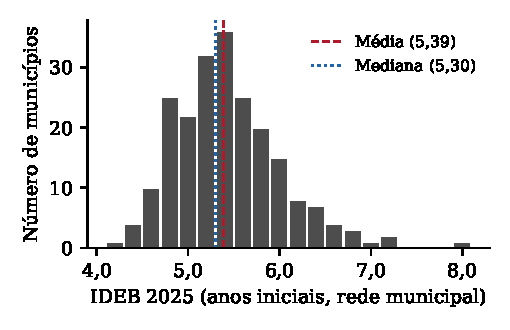
\includegraphics[width=\linewidth]{distribuicao_ideb.pdf}
    \caption{Distribuição do IDEB 2025 dos 216 municípios maranhenses com indicador divulgado (rede municipal, anos iniciais do ensino fundamental), em classes de 0,2 ponto. As linhas verticais marcam a média (5,39) e a mediana (5,30). Fonte: elaboração própria com dados de \citet{inep2025}.}
    \label{fig:dist_ideb}
\end{figure}

A amplitude de 4,00 pontos (4,10 a 8,10) é expressiva, dado que o IDEB varia de 0 a 10. Isso indica que, mesmo dentro do Maranhão, estado homogeneamente vulnerável em termos nacionais, existe variabilidade interna substancial, o que justifica investigar os fatores associados aos destaques positivos. Responder a essa pergunta exige, primeiro, reduzir a influência do contexto por meio de uma segmentação explícita e, depois, comparar, dentro de cada grupo, os municípios de alto e baixo desempenho.

\subsection{QP1: segmentação socioeconômica dos municípios}

A clusterização \textit{K-Means} foi aplicada sobre a \textit{renda per capita} e a \textit{pobreza extrema} (padronizadas pela mediana e pelo intervalo interquartil), testando de 2 a 10 grupos, conforme descrito na metodologia.

A Figura~\ref{fig:elbow} apresenta as curvas de inércia (cotovelo) e de \textit{Silhouette Score}. O \textit{Silhouette Score} atinge o valor máximo em $k = 3$ (0,506), acima de $k = 2$ (0,489) e de $k = 4$ (0,456). A estabilidade \textit{bootstrap} confirma a escolha: o ARI médio é 0,812 em $k = 3$, contra 0,744 em $k = 2$ e 0,704 em $k = 4$. Os dois critérios apontam, portanto, para a mesma partição, que é ao mesmo tempo a mais bem separada e a mais estável sob reamostragem entre as testadas. A curva de inércia decresce de forma gradual e não oferece, por si só, um critério adicional.

\begin{figure*}[!ht]
    \centering
    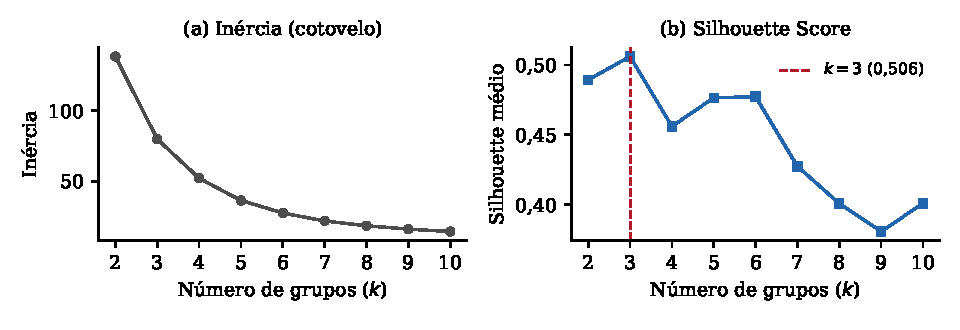
\includegraphics[width=0.85\linewidth]{elbow_silhouette.pdf}
    \caption{Escolha do número de \textit{clusters} para $k \in \{2, \ldots, 10\}$: (a) inércia intragrupo (Método do Cotovelo); (b) \textit{Silhouette Score} médio, com o máximo em $k = 3$ (0,506) marcado pela linha tracejada. Fonte: elaboração própria com dados de \citet{ibge2022, ibge2022classes}.}
    \label{fig:elbow}
\end{figure*}

A Figura~\ref{fig:pca} exibe os \textit{clusters} projetados nas duas primeiras componentes principais (a primeira componente, PC1, explica 93,6\% da variância; a segunda, PC2, explica 6,4\%). A predominância da primeira componente reflete a correlação entre as duas variáveis de segmentação: os municípios se distribuem essencialmente ao longo de um eixo de renda, no qual renda média alta e pobreza extrema baixa caminham juntas, e os três \textit{clusters} ocupam faixas sucessivas desse eixo.

\begin{figure}[!ht]
    \centering
    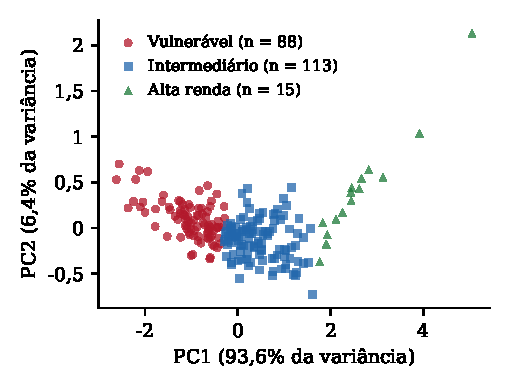
\includegraphics[width=\linewidth]{pca_clusters.pdf}
    \caption{Projeção dos 216 municípios maranhenses nas duas primeiras componentes principais, por \textit{cluster} socioeconômico ($k = 3$). Cada \textit{cluster} tem cor e marcador próprios. O eixo horizontal (PC1) concentra quase toda a variância e ordena os municípios da maior para a menor vulnerabilidade, da esquerda para a direita. Fonte: elaboração própria com dados de \citet{ibge2022, ibge2022classes}.}
    \label{fig:pca}
\end{figure}

O teste de ablação indica que as duas variáveis contribuem para a partição, com peso maior para a renda média. Refazendo a clusterização sem a renda \textit{per capita}, a concordância com a partição original cai para um ARI de 0,379; sem a pobreza extrema, o ARI é de 0,688. A pobreza extrema, portanto, não é redundante: a retirada dessa variável reclassifica parte relevante dos municípios, o que confirma que ela acrescenta à renda média a informação sobre a base da distribuição de renda.

A Tabela~\ref{tab:clusters} resume os três \textit{clusters} obtidos, denominados pelo critério de renda média. O \textit{cluster} de alta renda reúne a capital e os principais polos regionais do estado: São Luís, São José de Ribamar, Paço do Lumiar, Imperatriz, Timon, Açailândia, Balsas, Santa Inês, Pedreiras, Presidente Dutra, Porto Franco, Estreito, Carolina, Fortaleza dos Nogueiras e Itinga do Maranhão.

\begin{table}[!ht]
    \caption{Perfil dos \textit{clusters} socioeconômicos (médias municipais). Fonte dos dados: \citet{ibge2022, ibge2022classes, inep2025, inep2026microdados, inep2026sinopse}; cálculos próprios.}
    \label{tab:clusters}
    \centering
    \begin{tblr}{%
        colspec = {X[l] r r r},
        cells   = {font=\small},
        row{1}  = {font=\small\bfseries},
        width   = \linewidth
        }
        \toprule
        Indicador & Vulnerável & Intermediário & Alta renda \\
        \midrule
        Municípios (n) & 88 & 113 & 15 \\
        Renda \textit{per capita} (R\$) & 555,84 & 732,06 & 1.082,44 \\
        Pobreza extrema (\%) & 41,8 & 27,5 & 15,3 \\
        IDEB 2025 & 5,29 & 5,42 & 5,78 \\
        Escolas com internet (\%) & 83,8 & 89,0 & 94,3 \\
        Escolas com biblioteca ou sala de leitura (\%) & 15,8 & 19,3 & 38,7 \\
        Docentes EFAI com ensino superior (\%) & 55,9 & 64,0 & 79,1 \\
        \bottomrule
    \end{tblr}
\end{table}

O \textit{cluster} de alta renda, com 15 municípios, não tem amostra suficiente para a análise intragrupo por quartis, que resultaria em quatro ou cinco municípios em cada extremo. A análise comparativa é, portanto, conduzida nos \textit{clusters} vulnerável e intermediário, que juntos reúnem 201 dos 216 municípios analisados.

Os percentuais médios das variáveis de infraestrutura e de formação docente acompanham o gradiente de renda. A \textit{conectividade à internet} cresce de 83,8\% das escolas municipais no \textit{cluster} vulnerável para 94,3\% no de alta renda. O acesso a \textit{biblioteca ou sala de leitura} é baixo nos dois primeiros grupos e mais que dobra no de alta renda. A proporção média de \textit{docentes EFAI com ensino superior} vai de 55,9\% a 79,1\%, diferença que antecipa uma das hipóteses testadas no estágio intragrupo. Em resposta à QP1, os municípios maranhenses se organizam em três \textit{clusters} socioeconômicos ordenados pela renda, em uma partição estável sob reamostragem para a qual as duas variáveis contribuem.

\subsection{QP2: fatores discriminantes dentro dos \textit{clusters}}

A Tabela~\ref{tab:mw} reúne as variáveis com $p < 0{,}10$ no teste de Mann-Whitney nos dois \textit{clusters} analisados; as diferenças entre proporções são expressas em pontos percentuais (p.p.).

\begin{table*}[!ht]
    \caption{Variáveis com diferença entre municípios de alto e de baixo IDEB nos \textit{clusters} vulnerável e intermediário (Mann-Whitney bicaudal, $p < 0{,}10$). Alto e Baixo: médias dos grupos de alto e de baixo IDEB; $\Delta$: diferença entre as médias; $U$: estatística de Mann-Whitney; $\delta$: delta de Cliff; $q$: valor $q$ de Benjamini-Hochberg sobre as catorze variáveis de cada \textit{cluster}. Fonte dos dados: \citet{inep2026microdados, inep2025, inep2026sinopse, ibge2022, ibge2022classes}; cálculos próprios em Python (SciPy).}
    \label{tab:mw}
    \centering
    \begin{tblr}{%
        colspec = {X[l] r r r r r r r},
        cells   = {font=\small},
        row{1}  = {font=\small\bfseries},
        width   = 0.92\linewidth
        }
        \toprule
        Variável & Alto & Baixo & $\boldsymbol{\Delta}$ & $\boldsymbol{U}$ & $\boldsymbol{\delta}$ & $\boldsymbol{p}$ & $\boldsymbol{q}$ \\
        \midrule
        \SetCell[c=8]{l}{\textit{Cluster vulnerável (alto: n = 24; baixo: n = 23)}} & & & & & & & \\
        Docentes com ensino superior (\%) & 60,6 & 49,0 & $+$11,6 p.p. & 373,5 & 0,35 & 0,039 & 0,34 \\
        Docentes com licenciatura (\%)    & 59,1 & 47,8 & $+$11,4 p.p. & 369,0 & 0,34 & 0,049 & 0,34 \\
        \midrule
        \SetCell[c=8]{l}{\textit{Cluster intermediário (alto: n = 34; baixo: n = 29)}} & & & & & & & \\
        Escolas com quadra esportiva (\%)             & 12,9 & 5,4  & $+$7,5 p.p.  & 699,5 & 0,42 & 0,004 & 0,052 \\
        Turmas de correção de fluxo, anos finais (\%) & 0,90 & 0,07 & $+$0,8 p.p.  & 622,0 & 0,26 & 0,007 & 0,052 \\
        Docentes com ensino superior (\%)             & 69,2 & 58,1 & $+$11,1 p.p. & 637,5 & 0,29 & 0,047 & 0,18 \\
        Docentes com licenciatura (\%)                & 67,4 & 57,4 & $+$10,1 p.p. & 635,0 & 0,29 & 0,051 & 0,18 \\
        Renda \textit{per capita} (R\$)               & 753,15 & 719,13 & $+$34,02 & 620,0 & 0,26 & 0,081 & 0,23 \\
        \bottomrule
    \end{tblr}
\end{table*}

\subsubsection{\textit{Cluster} vulnerável}

Dentro do \textit{cluster} vulnerável (n = 88), os 24 municípios que se encontram no quartil superior de IDEB (alto, $\geq 5{,}60$, média 6,08) são comparados aos 23 do quartil inferior (baixo, $\leq 4{,}80$, média 4,61). A diferença média de 1,47 ponto de IDEB entre os grupos é substancial: equivale a quase dois desvios-padrão e meio da distribuição estadual.

A formação docente é a única dimensão que diferencia os municípios de alto e baixo IDEB no \textit{cluster} vulnerável. Os municípios de IDEB alto têm, em média, 11,6 p.p. a mais de \textit{docentes com ensino superior} e 11,4 p.p. a mais com \textit{licenciatura}, diferenças de efeito médio ($\delta$ de 0,35 e 0,34). Isoladamente, porém, esses testes não resistem à correção para comparações múltiplas ($q = 0{,}34$). A correlação de Spearman com todos os 88 municípios do \textit{cluster}, sem o descarte do intervalo central, confirma a associação com mais força: $\rho = 0{,}29$ para docentes com ensino superior ($p = 0{,}007$; $q = 0{,}063$) e $\rho = 0{,}28$ para licenciatura ($p = 0{,}009$; $q = 0{,}063$). Nenhuma outra variável mantém associação com o IDEB no \textit{cluster} após a correção ($q > 0{,}40$ em todas). Com a formação docente medida apenas na rede municipal, a associação se mantém e fica mais forte ($\delta$ de 0,38 e 0,42; $\rho$ de 0,32 e 0,35; $p \leq 0{,}026$), o que indica que a inclusão de docentes de outras redes na Sinopse não explica o resultado.

As duas variáveis se sobrepõem em grande parte (quase todos os docentes com ensino superior são licenciados) e devem ser lidas como um único achado. Ele dialoga com a literatura sobre o papel do professor \citep{rivkin2005} e com a meta nacional de formação em licenciatura \citep{brasil2014}, mas mede titulação, e não qualidade docente, e o faz no agregado municipal. \citet{rivkin2005} analisaram professores e alunos e encontraram pouca relação entre a titulação e o aprendizado, e a revisão de \citet{glewwe2013} chega a conclusão semelhante para países em desenvolvimento, nos estudos de maior rigor metodológico. Uma leitura possível é que, em redes nas quais mais de 40\% dos docentes ainda não concluíram a graduação, como as do \textit{cluster} vulnerável, a titulação diferencie os municípios mais do que em contextos em que ela já é quase universal.

A renda \textit{per capita} e a pobreza extrema não diferenciam os grupos de alto e baixo IDEB dentro desse \textit{cluster} ($p = 0{,}322$ e $p = 0{,}463$). Esse resultado é compatível com o propósito da segmentação: dentro do grupo, não se detecta diferença de renda entre os municípios de alto e de baixo IDEB. A ausência de significância, porém, não demonstra equivalência, sobretudo com grupos de 23 e 24 municípios, e diferenças socioeconômicas não captadas pela renda podem persistir.

\subsubsection{\textit{Cluster} intermediário}

Dentro do \textit{cluster} intermediário (n = 113), os 34 municípios do quartil superior de IDEB (alto, $\geq 5{,}70$, média 6,07) são comparados aos 29 do quartil inferior (baixo, $\leq 5{,}00$, média 4,81).

A formação docente reaparece no \textit{cluster} intermediário com magnitude semelhante à observada entre os municípios vulneráveis: 11,1 p.p. a mais de \textit{docentes com ensino superior} e 10,1 p.p. a mais com \textit{licenciatura} nos municípios de IDEB alto, com efeito médio ($\delta = 0{,}29$). A correlação de Spearman com todos os 113 municípios aponta na mesma direção ($\rho = 0{,}21$ e $0{,}20$; $p = 0{,}027$ e $0{,}036$), embora sem resistir à correção ($q$ de 0,12 e 0,13). A medida restrita à rede municipal reproduz o resultado com efeitos maiores ($\delta$ de 0,38 e 0,35; $p \leq 0{,}018$). Nenhum desses testes, isoladamente, é conclusivo; o que sustenta o achado é a sua repetição, com a mesma direção e magnitude, em dois grupos socioeconômicos distintos e nos dois procedimentos de comparação. Isso sugere que a associação entre formação docente e desempenho não se restringe a um único contexto socioeconômico.

A \textit{quadra esportiva} apresenta a diferença mais expressiva do \textit{cluster} ($p = 0{,}004$; $q = 0{,}052$; $\delta = 0{,}42$): as escolas com quadra são mais que o dobro nos municípios de IDEB alto (12,9\% contra 5,4\%), e a associação se mantém com todos os municípios do \textit{cluster} ($\rho = 0{,}23$; $q = 0{,}090$). Como a medida é municipal, o resultado não indica um efeito da atividade esportiva sobre os alunos. A presença de quadras pode sinalizar um padrão mais amplo de investimento da rede em infraestrutura escolar, leitura compatível com estudos que associam a infraestrutura ao IDEB, sobretudo nos anos iniciais \citep{alves2013, vasconcelos2021}; a análise, porém, não permite distinguir entre essas leituras. A proporção de turmas de correção de fluxo nos anos finais também é maior nos municípios de IDEB alto ($p = 0{,}007$; $q = 0{,}052$), mas os valores são pequenos (menos de 1\% das turmas), o efeito é pequeno ($\delta = 0{,}26$), e o resultado não permite inferir se a oferta de correção de fluxo é causa ou consequência do desempenho.

Diferentemente do \textit{cluster} vulnerável, a renda \textit{per capita} ainda apresenta diferença marginal entre os grupos ($p = 0{,}081$), de R\$~34 em média, o que indica alguma heterogeneidade residual de renda no \textit{cluster} intermediário, o maior dos três.

\subsubsection{Poder preditivo das variáveis}

As diferenças identificadas nos extremos de desempenho não se traduzem em capacidade de previsão. Em validação cruzada, o classificador \textit{Random Forest} não separou os municípios de alto e de baixo IDEB melhor que o acaso (AUC de 0,51 no \textit{cluster} vulnerável e de 0,57 no intermediário). A regressão \textit{ridge} não previu o IDEB melhor que a média, nem no estado como um todo ($R^2 = -0{,}01$), nem dentro dos \textit{clusters} ($R^2$ de $-0{,}10$ e $-0{,}07$). Os fatores discriminantes descritos acima são, portanto, associações específicas e de magnitude modesta: a maior parte da variação do IDEB entre municípios depende de fatores que as variáveis administrativas disponíveis não captam.

Em resposta à QP2, a formação docente é o fator que diferencia os municípios de alto e de baixo IDEB nos dois \textit{clusters} analisados, com efeito médio e de forma consistente entre procedimentos; no \textit{cluster} intermediário, somam-se a quadra esportiva e, com efeito pequeno, a correção de fluxo. Nenhum desses fatores, isoladamente ou em conjunto, prevê o desempenho.

\subsection{Diálogo com a literatura}

Os achados dialogam com a literatura de maneiras específicas. A centralidade da qualificação docente, observada nos dois \textit{clusters} com diferenças de 10 a 12 p.p. entre municípios de alto e baixo IDEB, é compatível com a ênfase da literatura no papel do professor \citep{rivkin2005} e com a prioridade que a política nacional atribui à formação em licenciatura \citep{brasil2014, gatti2019}. Vale a ressalva já apontada: o estudo mede a titulação no agregado das redes municipais, e não a qualidade de cada docente. A pesquisa em eficácia escolar \citep{brooke2008} oferece o enquadramento para esse resultado: controlado o contexto socioeconômico, parte da diferença de desempenho entre redes se associa a características das próprias redes escolares. A ausência de diferença significativa de renda e de pobreza extrema dentro do \textit{cluster} vulnerável é consistente com a tese de \citet{coleman1966} de que o contexto socioeconômico explica a maior parte da variação do desempenho. Quando esse contexto é aproximadamente controlado, as diferenças que restam passam a se associar a fatores escolares, de magnitude menor.

Em relação à literatura de mineração de dados educacionais, o trabalho contribui com uma aplicação metodológica que responde a duas limitações apontadas na Seção~\ref{sec:relacionados}: o uso de modelos globais que ignoram a heterogeneidade socioeconômica entre municípios e a menor presença de estudos sobre o Norte e o Nordeste. Em vez de produzir perfis como resultado final \citep{alves2014}, o agrupamento definiu os grupos de comparação do segundo estágio, e a validação da partição por \textit{Silhouette}, estabilidade e ablação dá transparência a essa etapa. A abordagem em dois estágios é replicável para outros estados e pode ser adaptada a outros níveis de ensino (anos finais do ensino fundamental, ensino médio) ou a outras medidas de desempenho. O baixo poder preditivo, por sua vez, é um resultado relevante para a área: modelos supervisionados treinados apenas com variáveis do Censo Escolar dificilmente separarão redes de alto e de baixo desempenho dentro de um mesmo contexto socioeconômico.

Quanto ao IDEB como métrica, os pressupostos estatísticos identificados por \citet{soares2013}, especialmente a correlação entre fluxo e proficiência, não invalidam a análise, mas sugerem cautela na interpretação: municípios com IDEB elevado podem estar priorizando aprovação em detrimento da proficiência. A inclusão de variáveis de fluxo (\textit{distorção idade-série}, \textit{correção de fluxo}) entre as explicativas não elimina esse risco: como o próprio IDEB incorpora a taxa de aprovação, essas variáveis guardam relação parcialmente mecânica com a variável-alvo, e as diferenças observadas nelas devem ser lidas com essa ressalva.

\subsection{Implicações para as políticas educacionais}

Os resultados têm implicações para gestores municipais e formuladores de políticas educacionais do Maranhão:

\begin{itemize}
  \item \textbf{Formação e habilitação docente (\textit{clusters} vulnerável e intermediário).} A diferença de 10 a 12 p.p. na proporção de \textit{docentes com ensino superior} entre municípios de alto e baixo IDEB se repete nos dois grupos analisados. Isso torna programas de formação continuada e de indução à licenciatura específica candidatos plausíveis de política pública em todo o estado, e não apenas nos municípios mais pobres. A análise associativa não permite, porém, quantificar o impacto esperado. Políticas de financiamento de graduação para docentes em exercício, como o Programa Nacional de Formação de Professores da Educação Básica (Parfor), são instrumentos já existentes cuja ampliação pode ser considerada, com avaliação de impacto que confirme o efeito sobre o desempenho.

  \item \textbf{Infraestrutura escolar (\textit{cluster} intermediário).} A quadra esportiva ($p = 0{,}004$; $q = 0{,}052$; $\delta = 0{,}42$) destaca-se como fator discriminante nos municípios de renda intermediária, sugerindo que, nesse grupo, o investimento em infraestrutura física complementar é candidato a priorização no monitoramento e na alocação orçamentária, ainda que a análise não permita estimar o retorno esperado desse investimento.

  \item \textbf{Monitoramento por perfil socioeconômico.} A segmentação permite que as redes se comparem com municípios de contexto semelhante, e não com médias estaduais ou nacionais. Municípios de IDEB alto dentro de cada \textit{cluster} podem servir de referência para os demais do mesmo grupo.
\end{itemize}

\section{Limitações da Pesquisa}
\label{sec:limitations}

As limitações deste estudo são organizadas segundo a taxonomia de validade de \citet{Wohlin2012} e devem ser consideradas na interpretação dos resultados.

\textbf{Validade interna.} A análise é descritiva e associativa, não causal. Não é possível afirmar que a \textit{formação docente} ou a \textit{infraestrutura escolar} causam IDEB mais alto. Municípios com gestão mais eficaz tendem a contratar mais docentes qualificados e a obter melhores resultados ao mesmo tempo, o que torna difícil separar o efeito de cada variável do efeito da qualidade de gestão municipal. A segmentação reduz o confundimento pela renda, mas não o elimina: no \textit{cluster} intermediário, a renda \textit{per capita} ainda difere marginalmente entre os grupos de alto e de baixo IDEB.

\textbf{Validade externa.} Os resultados se referem aos municípios maranhenses, à rede municipal, aos anos iniciais do ensino fundamental e à edição 2025 do IDEB. A transposição para outros estados exige replicar o procedimento, e não apenas os achados. Os 15 municípios de alta renda, que reúnem a capital e os principais polos regionais, não têm amostra suficiente para a comparação por quartis, e os fatores associados ao desempenho nesse grupo permanecem sem investigação.

\textbf{Validade de construto.} As duas variáveis de segmentação descrevem a distribuição de renda e são correlacionadas entre si ($-0{,}87$). Dimensões socioeconômicas não monetárias, como a escolaridade dos adultos e as condições de saúde, não entram na segmentação; a ablação mostra que a pobreza extrema acrescenta informação à renda média, mas a partição ainda é essencialmente ordenada ao longo de um eixo de renda. A titulação é uma medida indireta da qualidade docente, e a presença de quadra, uma medida indireta do investimento em infraestrutura. As variáveis são agregados municipais, e as associações valem para as redes municipais, não para escolas, professores ou alunos \citep{robinson1950}. A formação docente da Sinopse inclui os docentes de todas as redes do município; a verificação feita apenas com a rede municipal, que reúne 93\% a 95\% desses docentes nos grupos analisados, reproduz os resultados. Por fim, o próprio IDEB incorpora a aprovação, o que cria relação parcialmente mecânica com as variáveis de fluxo \citep{soares2013}.

\textbf{Validade de conclusão.} As comparações envolvem grupos de 23 a 34 municípios, o que limita o poder estatístico. Com a correção para comparações múltiplas, apenas a quadra esportiva e a correção de fluxo no \textit{cluster} intermediário mantêm valor $q$ próximo de 0,05. A formação docente é sustentada pela consistência entre os dois \textit{clusters} e entre os dois procedimentos de comparação, e não por um teste isolado, e os resultados devem ser lidos como exploratórios. Os modelos preditivos treinados com as variáveis do estudo não superaram o acaso na separação dos grupos nem a média na previsão do IDEB. O Censo Escolar não captura processos pedagógicos, gestão, clima escolar ou engajamento familiar, que são mediadores importantes do desempenho e provavelmente respondem pela maior parte da variação não explicada.

\section{Conclusão e Trabalhos Futuros}
\label{sec:conclusion}

Este trabalho propôs e aplicou uma abordagem em dois estágios (segmentação socioeconômica por \textit{K-Means} seguida de comparação intragrupo pelo teste de Mann-Whitney) aos 216 municípios maranhenses com dados no IDEB 2025 (anos iniciais do ensino fundamental, rede municipal). O problema que a motivou é conhecido na literatura: comparar municípios de contextos muito distintos tende a atribuir à escola diferenças que vêm da renda.

Quanto à QP1, a segmentação, feita com a renda \textit{per capita} e a proporção de moradores em pobreza extrema do Censo Demográfico 2022, produziu três grupos (vulnerável, intermediário e de alta renda). Essa partição foi escolhida tanto pelo \textit{Silhouette Score} quanto pela estabilidade \textit{bootstrap}, e as duas variáveis contribuem para ela. Quanto à QP2, nos dois grupos com amostra suficiente para a análise intragrupo, a \textit{formação docente} (proporção de professores com ensino superior e com licenciatura) está associada ao desempenho de forma consistente. As diferenças entre os municípios de alto e baixo IDEB são de 10 a 12 pontos percentuais, com efeito médio. No grupo intermediário, a presença de quadra esportiva também se destaca. O poder preditivo conjunto das variáveis, porém, é baixo.

Para gestores e formuladores de políticas, os resultados apontam a formação docente como fator associado ao desempenho de forma recorrente em municípios de renda baixa e intermediária, o que pode subsidiar a discussão sobre a alocação de recursos educacionais em diferentes perfis socioeconômicos. Para a pesquisa em informática na educação, o estudo mostra o uso do agrupamento como etapa de controle de contexto, validada por critérios de separação, estabilidade e ablação, combinada a testes não paramétricos com tamanho de efeito e correção para comparações múltiplas. O procedimento usa apenas dados públicos e \textit{scripts} abertos e pode ser replicado em outras unidades da federação.

Os trabalhos futuros decorrem das limitações identificadas. O primeiro é incorporar à segmentação dimensões não monetárias, como a escolaridade dos adultos, e comparar o \textit{K-Means} com outros algoritmos de agrupamento. O segundo é replicar o procedimento em outros estados do Nordeste e em outras etapas de ensino, o que permitiria também analisar os municípios de alta renda com amostra suficiente. O terceiro é verificar se a ampliação da formação docente eleva o desempenho, o que exige estudos com desenho longitudinal ou quase experimental, com as próximas edições do IDEB e do Censo Escolar.

\begin{declarations}

\begin{contributions}
\ifidentificado
DJC: concepção do estudo, metodologia, curadoria dos dados, \textit{software} (\textit{scripts} de análise), análise formal, visualização e redação do manuscrito (rascunho original, revisão e edição). ODRF e DSP: supervisão, revisão crítica do manuscrito (revisão e edição) e aprovação da versão final. Todas as pessoas autoras leram e aprovaram o manuscrito final.
\else
Omitido para revisão.
\fi
\end{contributions}

\begin{interests}
As pessoas autoras declaram que não têm nenhum conflito de interesses.
\end{interests}

\begin{materials}
Os dados analisados são públicos e foram obtidos do INEP (IDEB 2025, microdados do Censo Escolar 2025 e Sinopse Estatística da Educação Básica 2025) e do IBGE (Censo Demográfico 2022, Sidra, tabelas 10295 e 10296). Os \textit{scripts} de ingestão, transformação e análise, com instruções de execução e o ambiente Python reprodutível, estão disponíveis em
\ifidentificado
\url{https://github.com/darlondjc/desempenho-educacional-maranhao}.
\else
repositório anonimizado para a revisão: \url{https://anonymous.4open.science/r/desempenho-educacional-maranhao-97FB/}.
\fi
\end{materials}

\begin{aiusagedeclaration}
Foram utilizadas ferramentas de inteligência artificial generativa nas seguintes etapas: o Claude (Anthropic), na correção e revisão dos \textit{scripts} Python da análise, com cada alteração validada pela autoria; o Claude e o ChatGPT (OpenAI), na revisão da redação e da clareza do texto; o Claude e o SciSpace AI Research (PubGenius Inc.), na busca de trabalhos relevantes e na verificação de metadados de citações, com cada referência conferida na fonte original; e o Claude, na adaptação do manuscrito ao modelo da RBIE, o que incluiu a reorganização das seções, a tradução dos resumos e a redação de versões preliminares de trechos de ligação a partir do conteúdo produzido pela autoria, todos revisados pelas pessoas autoras. Os dados, a análise e a interpretação dos resultados não foram gerados por essas ferramentas. Elas não figuram como autoras, e as pessoas autoras assumem integral responsabilidade por todo o conteúdo do manuscrito.
\end{aiusagedeclaration}

\begin{furtherinformation}
O estudo usa apenas dados secundários públicos, agregados por município, e dispensa apreciação por Comitê de Ética em Pesquisa (ver Seção~\ref{sec:metodos}).
\end{furtherinformation}

\end{declarations}


\bibliographystyle{apalike-sol}
\bibliography{refs}

\end{document}
